% \section{Linear Regression for Multivariate Real World Data  $\And$ Bivariate Data}
% The model implemented here makes use of a Gaussian Basis Function,
% \begin{equation*}
%     \mathbb{\phi}_j(\mathbf{x}) = \exp \left( {-\frac{(\mathbf{x} - \mu_j)^2}{\sigma^2}} \right)
% \end{equation*}


% \subsection{Experiments $\And$ Observations on Dataset 2:}



% \subsubsection{RMS error comparison for varying dimensions of $\mathbb{\phi}(\mathbf{x})$:}
% \parindent Only the dimension was changed here and variance was set to a constant value of 30 without any regularisation. As can be observed from the table[8], the $E_{rms}$ value of the training, validation and test data set decreases as the complexity of the model is increased. Also, there isn't much overfit when the dimensions are increased to 100 since there was enough data available.

% {\rowcolors{3}{green!40!yellow!10}{green!0!yellow!30}
% \begin{table}[hptb]
% \begin{tabular}{ |p{1.5cm}|p{3cm}|p{3cm}| p{3cm}|  }
% \hline
% \multicolumn{4}{|c|}{$\mathbf{E}_{rms}$ values for different data } \\
% \hline
% \rowcolor{lightgray} \textbf{Dimension} & $\mathbf{E}_{rms-train}$ & $\mathbf{E}_{rms-val}$ & $\mathbf{E}_{rms-test}$ \\
% \hline
%   2   &   20742.417961375482    &       19314.336433527136    &     20051.47268871791   \\
%  \hline
%  3   &   15755.436189348633    &       15039.506378963442    &     15602.040608854932   \\   
%  \hline
%  6   &   14465.019060036939    &       14170.647936247557    &     14146.981889693609         \\
%  \hline
%  9   &   9215.113706469303     &       9244.777763533128     &     8648.719452138206     \\
%  \hline
%  20  &   6043.52872279345      &       5996.571277859385     &     6128.169849741222     \\
%  \hline
%  30  &   4780.139930356894     &       4667.322597766088     &     4681.781287505215      \\
%  \hline
%  40  &   3250.5764084440207    &       3330.783324829522     &     3247.7191047865876     \\  
%  \hline
%  100 &   1454.005863919257     &       1609.951973441829     &     1580.1611713736224     \\
% \hline
% \end{tabular}
% \caption{Error comparisons for varying dimensions of $\phi(\mathbf{x}) $ for Dataset 2}
% \label{table:8}
% \end{table}
% }


% \subsubsection{RMS error comparison for varying variance of $\mathbb{\phi}(\mathbf{x})$:}

% Only the variance was changed here and dimensions were set to a constant value of 100 without any regularisation. The $E_{rms}$ decreases initially as the variance is increased and there isn't much change observed after a certain point. Table [9] demonstrates this.

% {\rowcolors{3}{green!40!yellow!10}{green!0!yellow!30}
% \begin{table}[hptb]
% \begin{tabular}{ |p{1.5cm}|p{3cm}|p{3cm}| p{3cm}|  }
% \hline
% \multicolumn{4}{|c|}{$\mathbf{E}_{rms}$ values for different data } \\
% \hline
% \rowcolor{lightgray} \textbf{Variance} & $\mathbf{E}_{rms-train}$ & $\mathbf{E}_{rms-val}$ & $\mathbf{E}_{rms-test}$ \\
% \hline
%   1   &   27266.067337673085     &       26794.717392625018       &     20051.47268871791   \\
%  \hline
%   10   &   3656.998466228972     &       3735.493387300531        &     3906.388733286057   \\   
%  \hline
%   20  &  3955.814282945206       &       4130.987734108473        &     4077.2036579847054        \\
%  \hline
%   30  &   3448.199977857502      &       3590.5182818874255       &     3441.4907182960355     \\
%  \hline
%   50  &   3344.7152080262267     &       3317.3693879440525       &     3299.934482599632     \\
%  \hline
%   100  &   3460.736021173579     &       3586.197518340341        &     3471.484357305657      \\
% \hline
% \end{tabular}
% \caption{Error comparisons for varying variance of $\phi(\mathbf{x}) $ for Dataset 2}
% \label{table:9}
% \end{table}
% }



% \subsubsection{RMS error comparison for varying regularisation parameters of quadratic regularisation:}

% Only the regularisation was changed here and dimensions were set to 100 with a variance of 30. The $E_{rms}$ increases as the regularisation parameter increases which tells that the model is now trying to reduce the overfit. As can be observed, the $E_{rms}$ of validation and test set is less than the $E_{rms}$ on the training set but it comes as a result of increase in overall $E_{rms}$. Table [10] demonstrates this.

% {\rowcolors{3}{green!40!yellow!10}{green!0!yellow!30}
% \begin{table}[hptb]
% \begin{tabular}{ |p{1.5cm}|p{3cm}|p{3cm}| p{3cm}|  }
% \hline
% \multicolumn{4}{|c|}{$\mathbf{E}_{rms}$ values for different data } \\
% \hline
% \rowcolor{lightgray}\textbf{$\lambda$} & $\mathbf{E}_{rms-train}$ & $\mathbf{E}_{rms-val}$ & $\mathbf{E}_{rms-test}$ \\
% \hline
%   0      &   1397.932974026646    &       1410.9028219564577       &     1545.4716845597673   \\
%  \hline
%   10e-5  &   3964.4172602252547    &       3870.2365010758563        &     3849.030700922454   \\   
%  \hline
%   10e-4  &  8711.736211556994       &       7773.878856448405        &     8852.914573070351        \\
%  \hline
%   10e-3  &   15352.219047826447      &       14113.981029840956       &     15308.868272544152     \\
%  \hline
%   10e-2  &   23555.54821056003      &       22613.32447875262       &     23171.93371145183    \\
%  \hline
%   10e-1  &   35560.49095521766     &       33790.609053408574        &     34783.161122408135      \\
%   \hline
%   10     &   38899.73825135093    &        36755.95627333107         &     38013.62049175868      \\
%   \hline
%   10e2   &   39374.00056336752    &         37152.40595020841       &      38408.5229340378        \\
%   \hline
%   10e3   &   39462.66115053631   &        37202.5849146428         &       38427.786409380235      \\
%   \hline
%   10e4   &   42522.79510032822   &         40234.01328931874       &        41188.57306560426      \\
%   \hline
%   10e5  &    51525.586833163274  &         49441.16118608065       &        50036.24559820878      \\
% \hline
% \end{tabular}
% \caption{Error comparisons for varying regularisation parameter of quadratic regularisation for Dataset 2}
% \label{table:10}
% \end{table}
% }

% \newpage
% \subsubsection{Scatter Plots of Best Model}

% Figure [\ref{fig:17}] shows the the scatter plot of predicted and actual target variable for the training and the test data.

% \begin{figure}[h]
%     \centering
%     \begin{subfigure}[t]{0.50\textwidth}
%         \centering
%         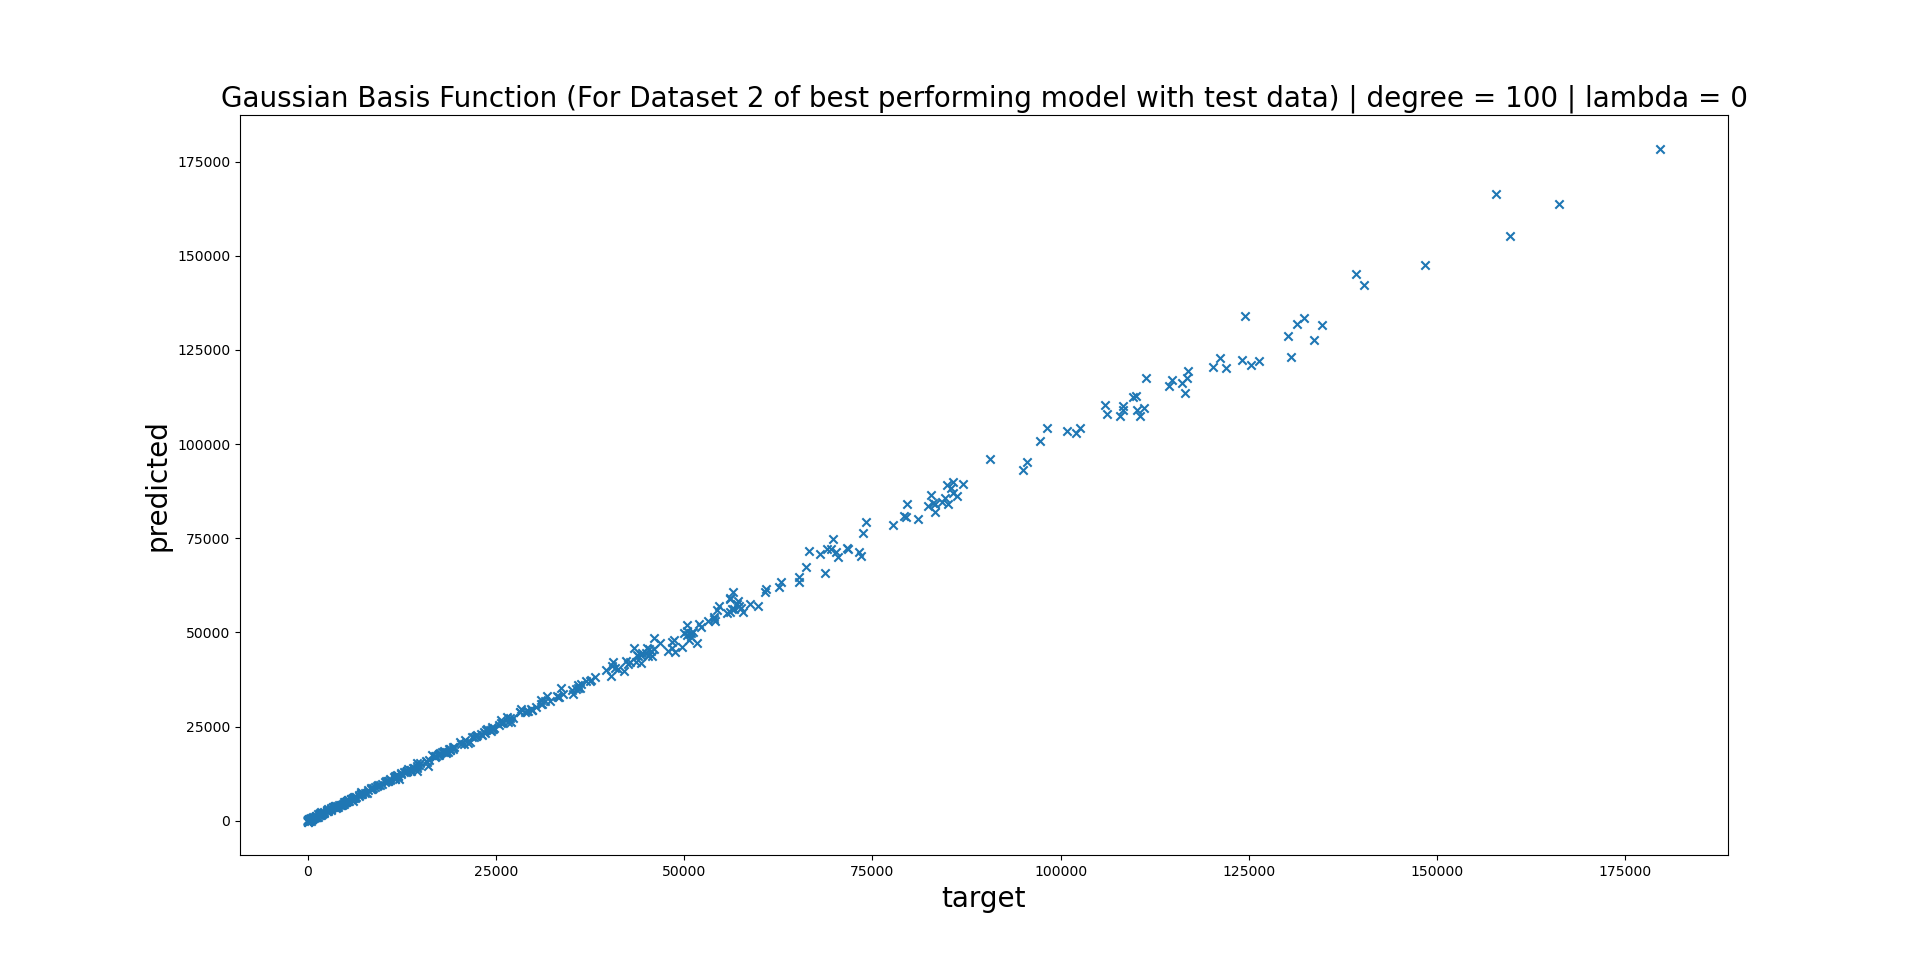
\includegraphics[height=1.6in]{Task 3 Images/3.1.42.png}
%         \caption{Training Data}
%     \end{subfigure}%
%     ~ 
%     \begin{subfigure}[t]{0.50\textwidth}
%         \centering
%         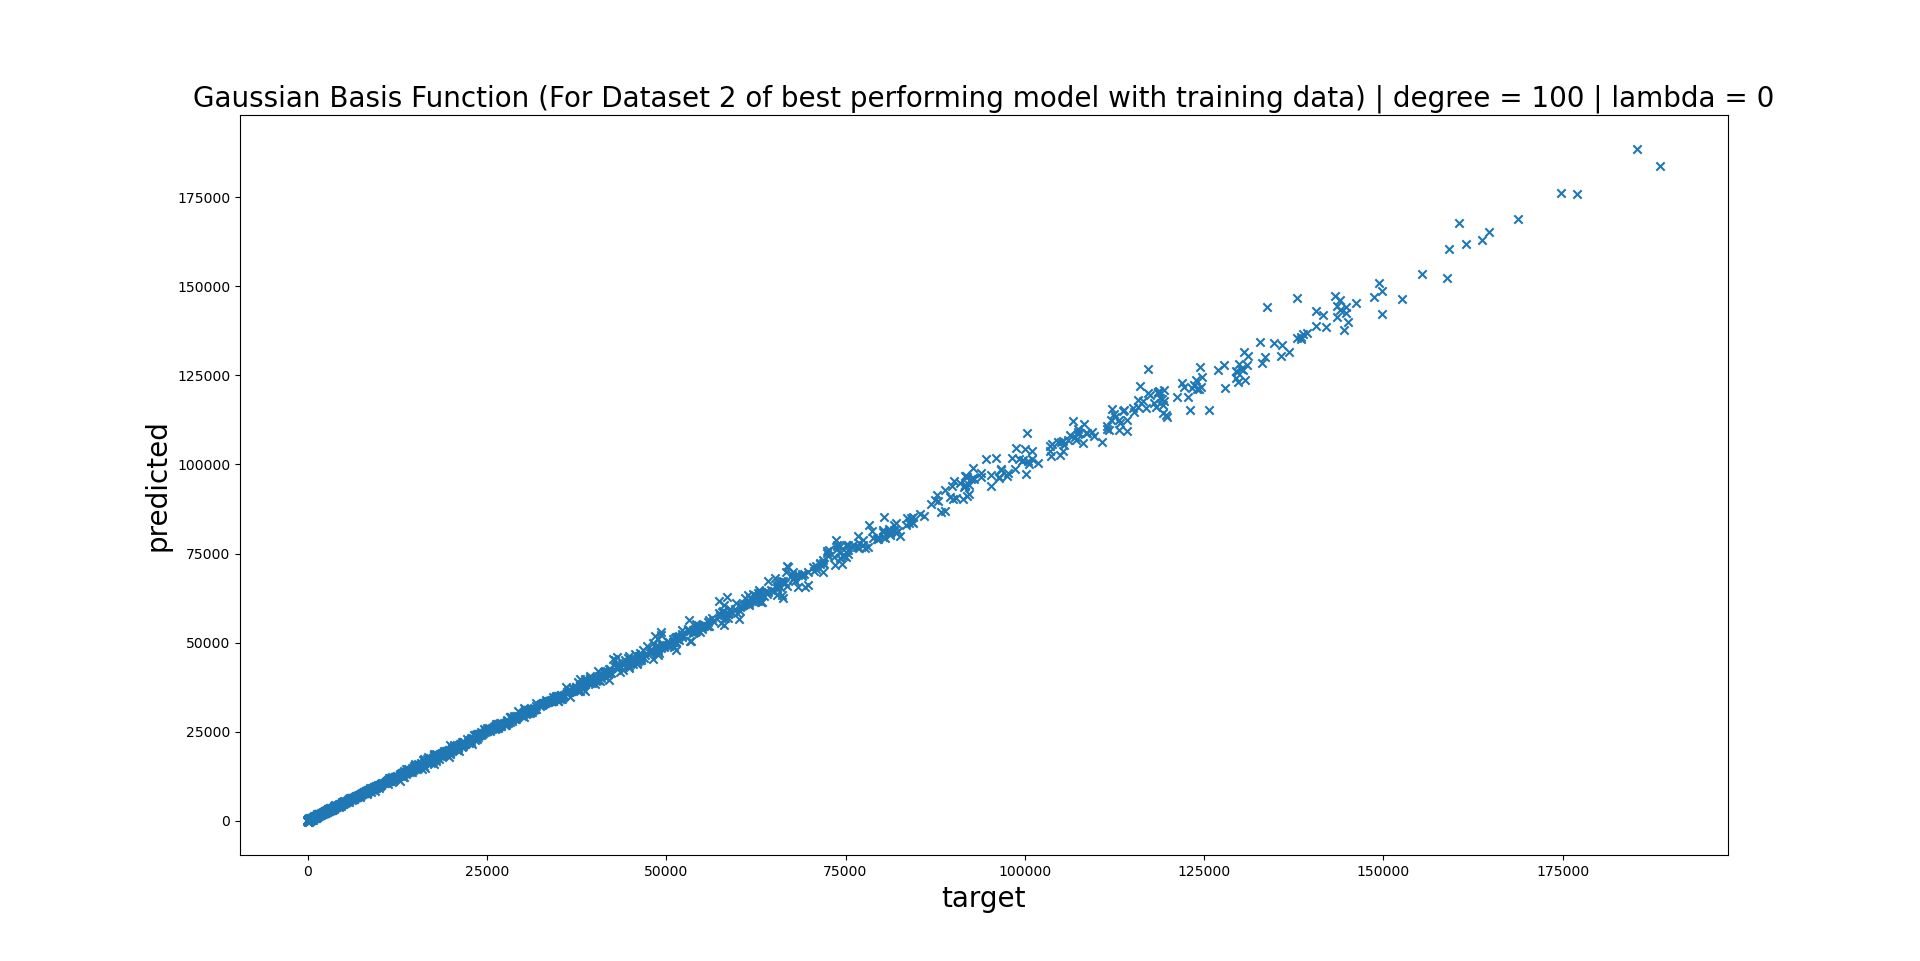
\includegraphics[height=1.6in]{Task 3 Images/3.1.41.png}
%         \caption{Test Data }
%     \end{subfigure}%
%     \caption{Scatter Plot of the Gaussian Basis Function of the best performing model for Dataset 2}
%     \label{fig:17}
% \end{figure}





%%%%%%%%%%%%%%%%%%%%%%%%%%%%%%%%%%%%%%%%%%%%%%%%%%%%%%%%%%%%%%%%%%%%%%%%%%%%%%%%%%%%%%%%%%%%%%%%%%%%%%%%%%%%%%%%%%%%%%%%%%%%%%%
\subsection{Experiments $\And$ Observations on Dataset 3:}

\begin{figure}[!ht]
    \centering
        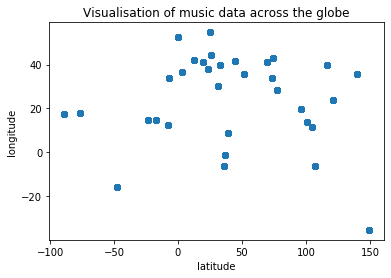
\includegraphics[height=3.2in]{Task 3 Images/Visualisation of music data across the globe.png}
        \caption{Training Data}
\end{figure}

\subsubsection{RMS error comparison for varying dimensions and width of $\mathbb{\phi}(\mathbf{x})$:}

A total of 500 samples from the given bivariate dataset was chosen at random anddivided  in  to  training,  validation  and  test  data(70\%,  20\%  and  10\%).   Using  the training data thus generated an attempt is made to find the best model.  At first the case without regularisation is considered.  For each dimension of the gaussian basis function, different values of width has been experimented here.  As can be concluded from the tables, a dimension of 100 with width of 10 seems to be the optimal model for the regression task at hand. Also one can observe overfitting when the dimensions are increased to 340. Here x,y in each column of the table represents the Erms in both the output dimensions

\newpage
{\rowcolors{3}{green!40!yellow!10}{green!0!yellow!30}
\begin{table}[hptb]
\begin{tabular}{ |p{1.5cm}|p{3cm}|p{3cm}| p{3cm}|  }
\hline
\multicolumn{4}{|c|}{$\mathbf{E}_{rms}$ values for dimension $25$ } \\
\hline
\rowcolor{lightgray} \textbf{Width} & $\mathbf{E}_{rms-train}$ & $\mathbf{E}_{rms-val}$ & $\mathbf{E}_{rms-test}$ \\
\hline
  1   &   17.19,48.11   &    19.49,52.58      &     16.25,47.46 \\
 \hline
 10   &   15.23,43.45  &  19.17,45.01          &     15.50,42.72 \\
 \hline
 50   &   15.01,42.80  & 19.52,45.40 & 15.16,46.30 \\
\hline
\end{tabular}
\label{table:8}
\end{table}
}

{\rowcolors{3}{green!40!yellow!10}{green!0!yellow!30}
\begin{table}[hptb]
\begin{tabular}{ |p{1.5cm}|p{3cm}|p{3cm}| p{3cm}|  }
\hline
\multicolumn{4}{|c|}{$\mathbf{E}_{rms}$ values for dimension $50$ } \\
\hline
\rowcolor{lightgray} \textbf{Width} & $\mathbf{E}_{rms-train}$ & $\mathbf{E}_{rms-val}$ & $\mathbf{E}_{rms-test}$ \\
\hline
  1   &   15.91,44.73   &    19.44,52.32      &     16.29,46.97 \\
 \hline
 10   &   13.82,40.69  &  19.32,45.60          &     13.56,42.47 \\
 \hline
 50   &   14.24,39.84  & 19.19,45.61 & 14.53,43.38 \\
\hline
\end{tabular}
\label{table:8}
\end{table}
}

{\rowcolors{3}{green!40!yellow!10}{green!0!yellow!30}
\begin{table}[hptb]
\begin{tabular}{ |p{1.5cm}|p{3cm}|p{3cm}| p{3cm}|  }
\hline
\multicolumn{4}{|c|}{$\mathbf{E}_{rms}$ values for dimension $100$ } \\
\hline
\rowcolor{lightgray} \textbf{Width} & $\mathbf{E}_{rms-train}$ & $\mathbf{E}_{rms-val}$ & $\mathbf{E}_{rms-test}$ \\
\hline
  1   &   13.21,42.71   &    19.21,46.37      &     19.88,48.96 \\
 \hline
 10   &   11.99,33.57  &  18.61,42.23          &     13.18,39.20 \\
 \hline
 50   &   12.12,33.54  & 22.19,46.99 & 14.34,45.70 \\
\hline
\end{tabular}
\label{table:8}
\end{table}
}

{\rowcolors{3}{green!40!yellow!10}{green!0!yellow!30}
\begin{table}[!h]
\begin{tabular}{ |p{1.5cm}|p{3cm}|p{3cm}| p{3cm}|  }
\hline
\multicolumn{4}{|c|}{$\mathbf{E}_{rms}$ values for dimension $340$ } \\
\hline
\rowcolor{lightgray} \textbf{Width} & $\mathbf{E}_{rms-train}$ & $\mathbf{E}_{rms-val}$ & $\mathbf{E}_{rms-test}$ \\
\hline
  1   &   1.73,6.06   &    23.07,68.55      &   22.38,62.18 \\
 \hline
 10   &   1.90,5.90  &  26.20,50.01          &   14.12,46.23 \\
 \hline
 50   &   2.23,5.98  & 26.04,57.54 & 23.33,66.33 \\
\hline
\end{tabular}
\label{table:8}
\end{table}
}

\newpage
\subsubsection{RMS error comparison for varying regularisation parameters of quadratic and Tikhonov regularisation}

Only the regularisation was changed here and dimensions were set to 100 with a variance of 3. The Erms increases as the regularisation parameter increases which tells that the model is now trying to reduce the overfit. As can be observed, the difference between $E_{rms}$ of validation and test set is less with the $E_{rms}$ on the training set is now less but it comes as a result of increase in overall $E_{rms}$. Table [\ref{table:14}] demonstrates this.

{\rowcolors{3}{green!40!yellow!10}{green!0!yellow!30}
\begin{table}[hptb]
\begin{tabular}{ |p{1.5cm}|p{3cm}|p{3cm}| p{3cm}|  }
\hline
\multicolumn{4}{|c|}{$\mathbf{E}_{rms}$ values for different data } \\
\hline
\rowcolor{lightgray} $\lambda$ & $\mathbf{E}_{rms-train}$ & $\mathbf{E}_{rms-val}$ & $\mathbf{E}_{rms-test}$ \\
\hline
  10e-5  &  $1.97$,$5.96$       &       $21.77$ ,$46.14$ & $11.34$, $41.73$  \\
 \hline
  10e-3  &   $5.79 $, $ 13.55$       &       $18.91$,$43.57$        &  $12.08$, $37.75$  \\
 \hline
  10e-1  &   $12.27$, $35.94$       &       $18.39$, $42.86$ & $13.56$,$38.78$  \\
 \hline
  0  &    $1.90$, $5.90$     &      $26.20$  $50.01 $         &     $14.12$,$46.23$ \\
  \hline
  10     &   $14.98$,  $43.41$   &        $18.58$,$45.88$         &     $15.10$,$43.18$     \\
  \hline
  10e+03   &   $21.92$, $55.43$    &         $22.41$,$59.02$      &      $21.42$,$53.03$        \\
  \hline
  10e+05  &    $32.75$, $63.30$  &         $31.42$,$67.81$       &        $31.97$,$61.44$      \\
\hline
\end{tabular}
\caption{Error comparisons for quadratic regularisation by varying $\lambda $  and fixed dimension =340 and width = 10 for Dataset 3}
\label{table:13}
\end{table}
}


{\rowcolors{3}{green!40!yellow!10}{green!0!yellow!30}
\begin{table}[hptb]
\begin{tabular}{ |p{1.5cm}|p{3cm}|p{3cm}| p{3cm}|  }
\hline
\multicolumn{4}{|c|}{$\mathbf{E}_{rms}$ values for different data } \\
\hline
\rowcolor{lightgray} \textbf{Variance} & $\mathbf{E}_{rms-train}$ & $\mathbf{E}_{rms-val}$ & $\mathbf{E}_{rms-test}$ \\
\hline
  10e-3  &   $2.37 $, $ 6.52$       &       $19.40$,$44.16$        &  $12.32$, $38.92$  \\
 \hline
  10e-1  &   $11.23$, $32.31$       &       $18.21$, $42.89$ & $12.95$,$38.52$  \\
 \hline
  0  &    $1.90$, $5.90$     &      $26.20$  $50.01 $         &     $14.12$,$46.23$ \\
  \hline
  10     &   $15.43$,  $44.86$   &        $18.59$,$48.12$         &     $14.89$,$44.27$     \\
  \hline
  10e+03   &   $32.06$, $62.60$    &         $30.76$,$67.07$      &      $31.26$,$60.72$        \\
  \hline
  10e+05  &    $33.10$, $63.58$  &         $31.73$,$68.11$       &        $32.33$,$61.74$      \\
\hline
\end{tabular}
\caption{Error comparisons for tikhonov regularisation by varying $\lambda $  and fixed dimension =340 and width = 10 for Dataset 3}
\label{table:14}
\end{table}
}

\newpage
\subsubsection{Scatter Plots of Best Model:}

Figure [\ref{fig:18}] shows the the scatter plot of predicted and actual target variable for the training and the test data.

\begin{figure}[h]
    \centering
    \begin{subfigure}[t]{0.50\textwidth}
        \centering
        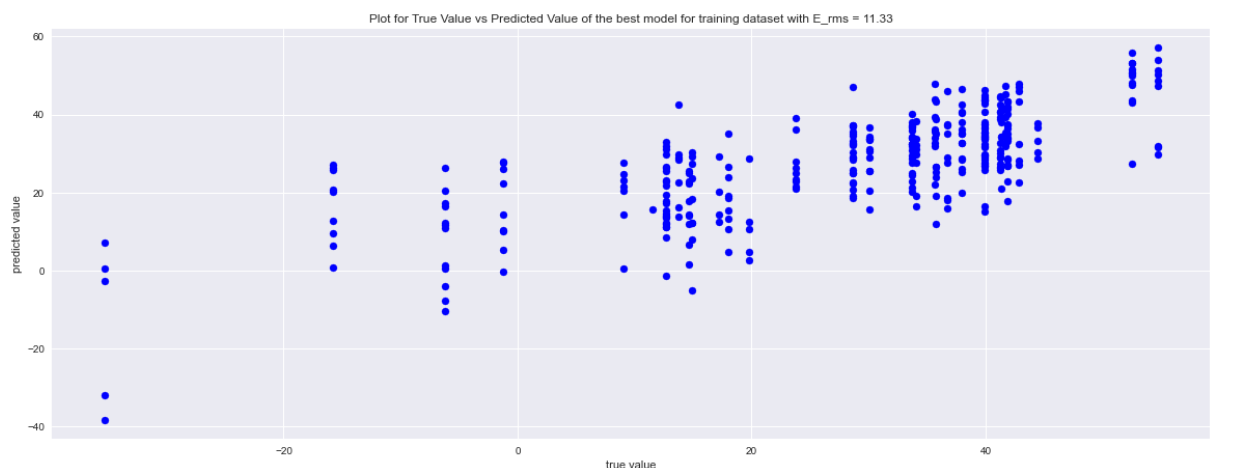
\includegraphics[height=1.6in]{Task3_new_images/rwd_tr_y0.png}
        \caption{Training Data}
    \end{subfigure}%
    ~ 
    \begin{subfigure}[t]{0.50\textwidth}
        \centering
        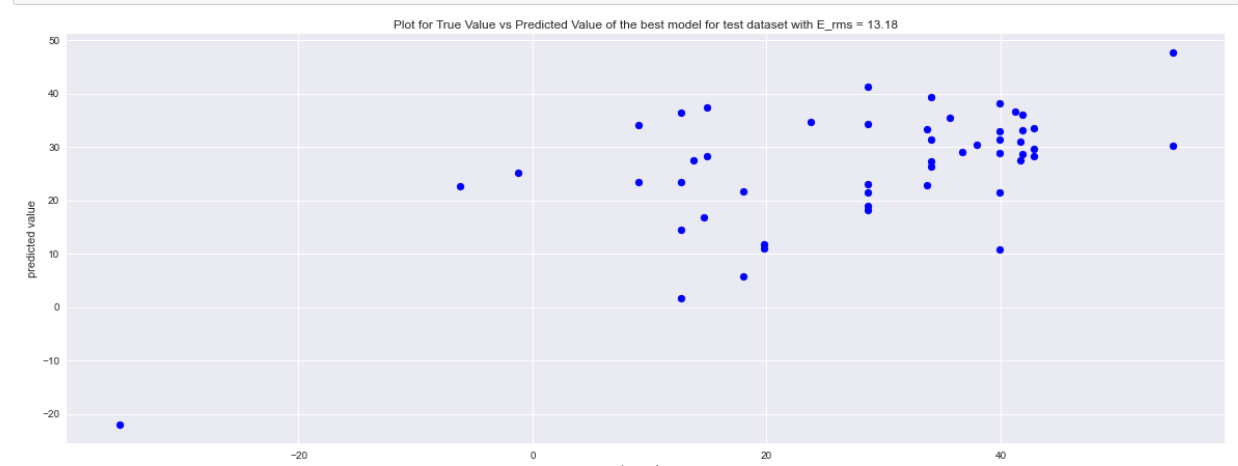
\includegraphics[height=1.6in]{Task3_new_images/rwd_test_y0.png}
        \caption{Test Data}
    \end{subfigure}%
    \caption{Scatter Plot of the Gaussian Basis Function of the best performing model for Dataset 3 for first column}
    \label{fig:18}
\end{figure}

\begin{figure}[h]
    \centering
    \begin{subfigure}[t]{0.50\textwidth}
        \centering
        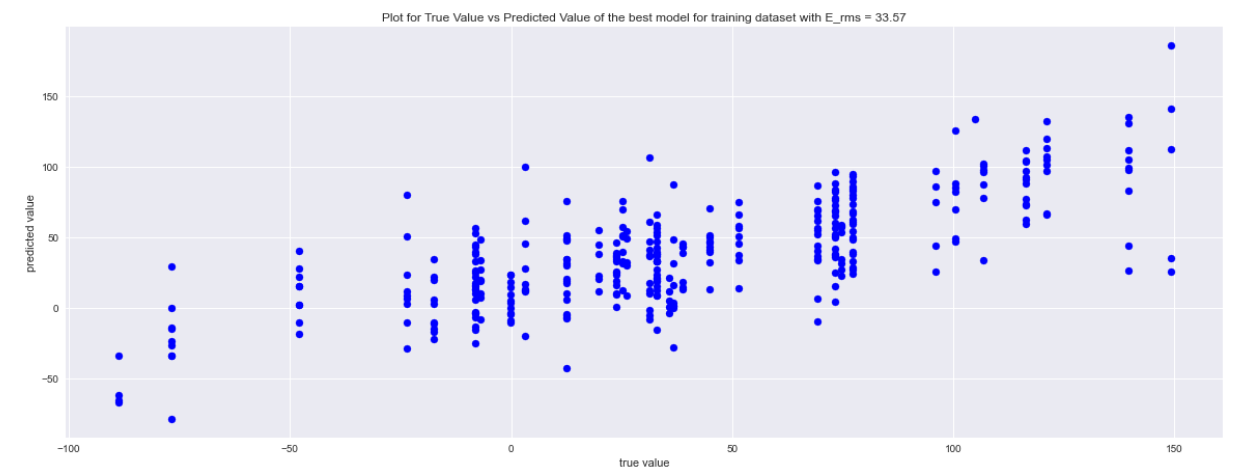
\includegraphics[height=1.6in]{Task3_new_images/rwd_tr_y1.png}
        \caption{Training Data}
    \end{subfigure}%
    ~ 
    \begin{subfigure}[t]{0.50\textwidth}
        \centering
        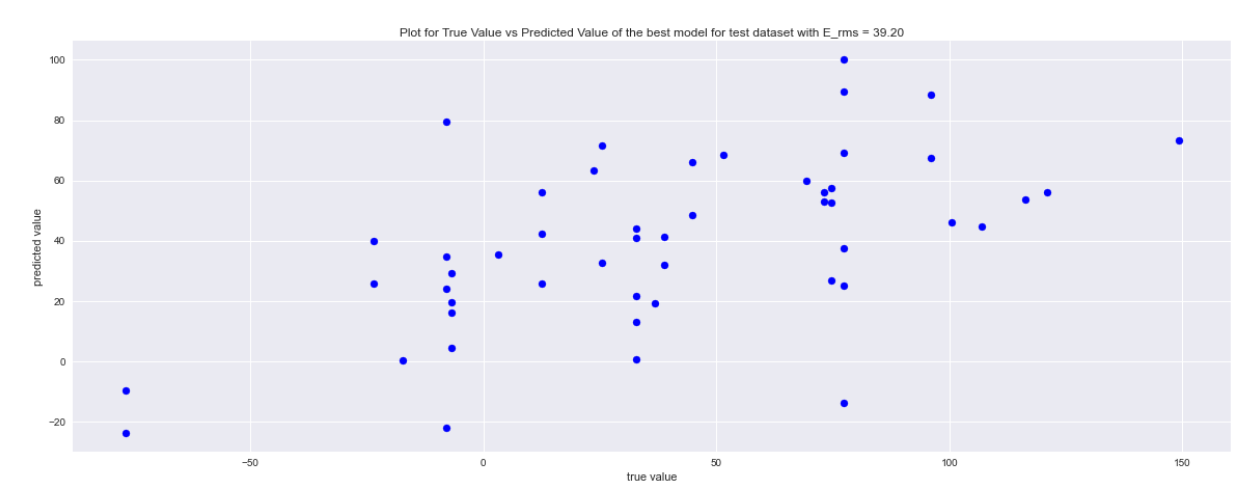
\includegraphics[height=1.6in]{Task3_new_images/rwd_test_y1 .png}
        \caption{Test Data}
    \end{subfigure}%
    \caption{Scatter Plot of the Gaussian Basis Function of the best performing model for Dataset 3 for second column}
    \label{fig:18}
\end{figure}

